\subsubsection{Esquema Entidad/Relación:}

\begin{figure}[h!]
	\centering
	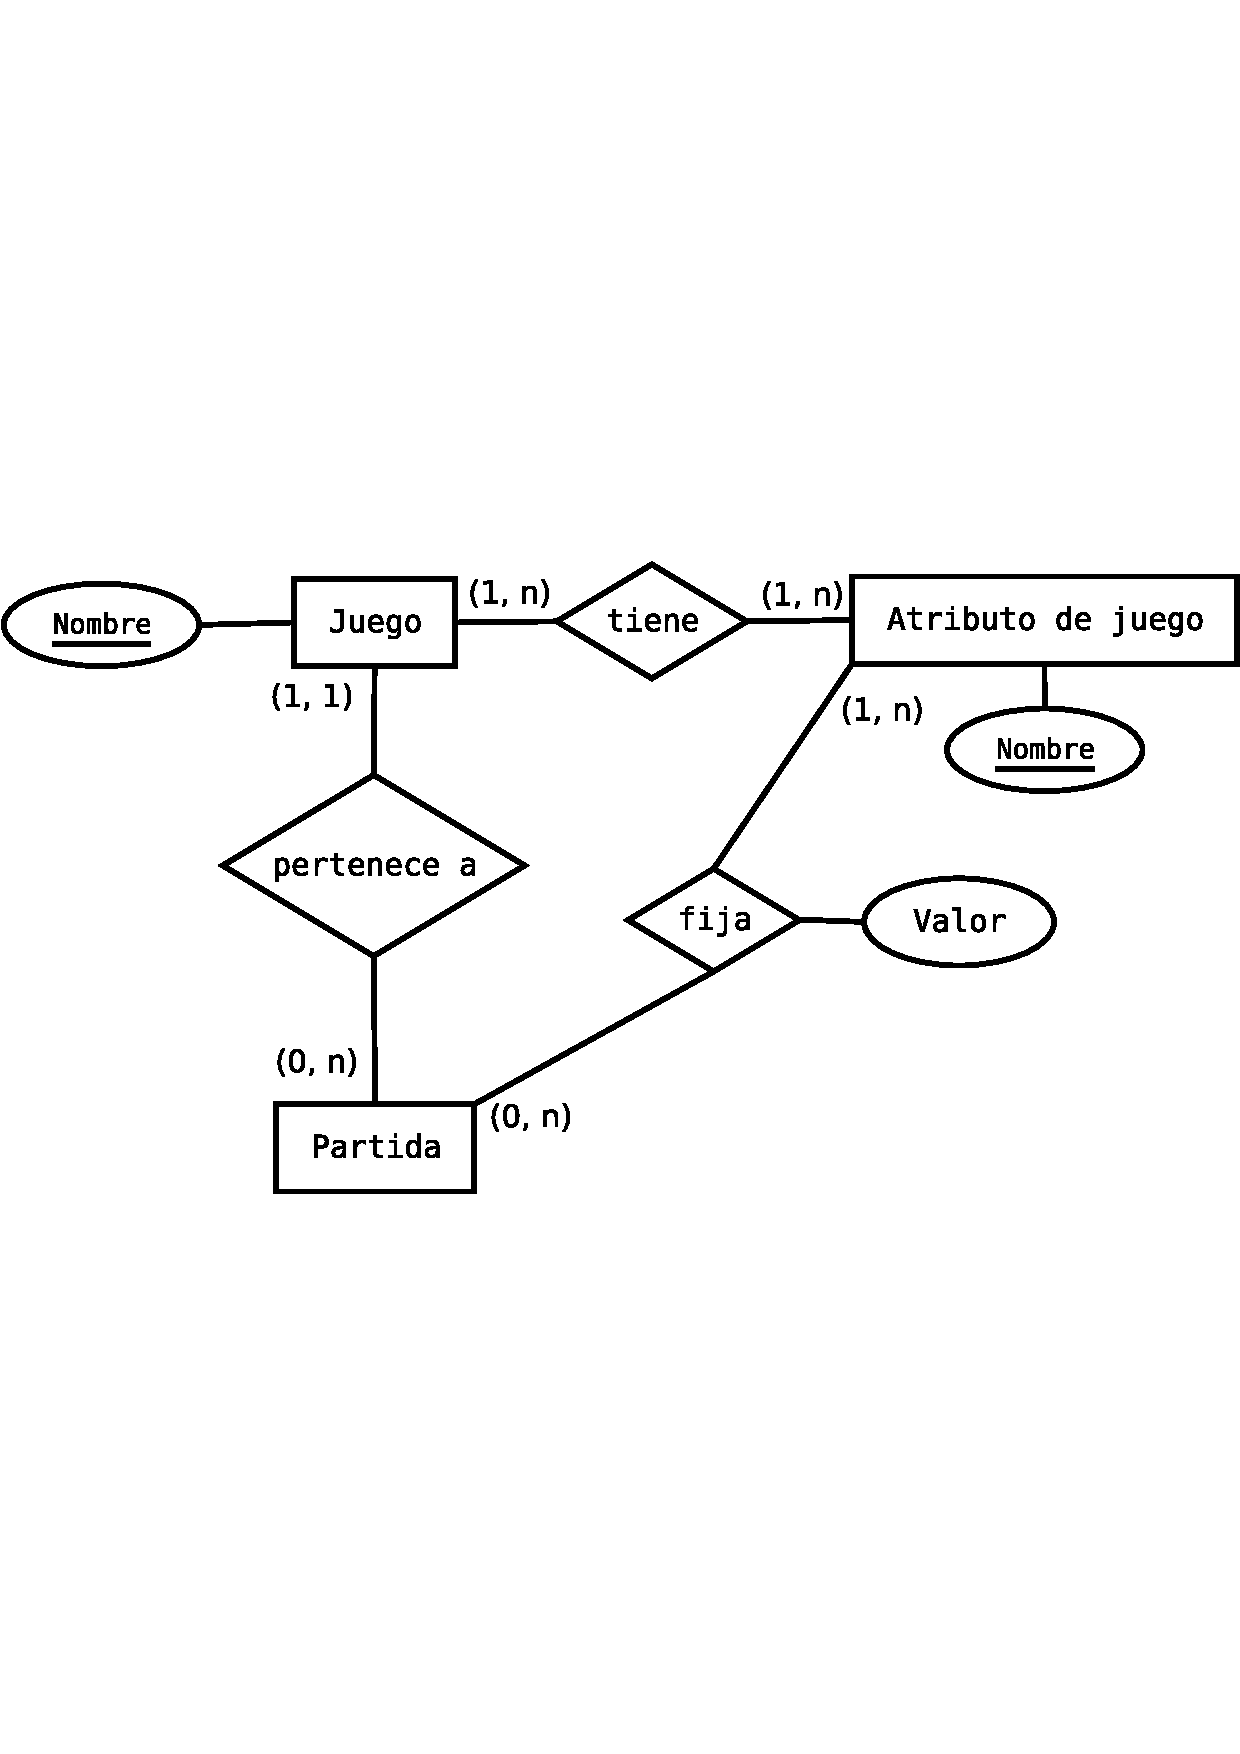
\includegraphics[width=0.7\linewidth]{../Diagramas/pdf/ER-Consulta.pdf}
	\caption{Flujo de datos del subsistema Consulta.}
	
	\label{fig:ERConsulta}
\end{figure}

\subsubsection{Diagramas de flujo de datos:}

Refinamos el proceso Consulta en sus cuatro requisitos funcionales  y realizando la descomposición del almacén en Partidas y Atributos mediante una primitiva descendente de descomposición en procesos sin conexiones.
 
\begin{figure}[h!]
\centering
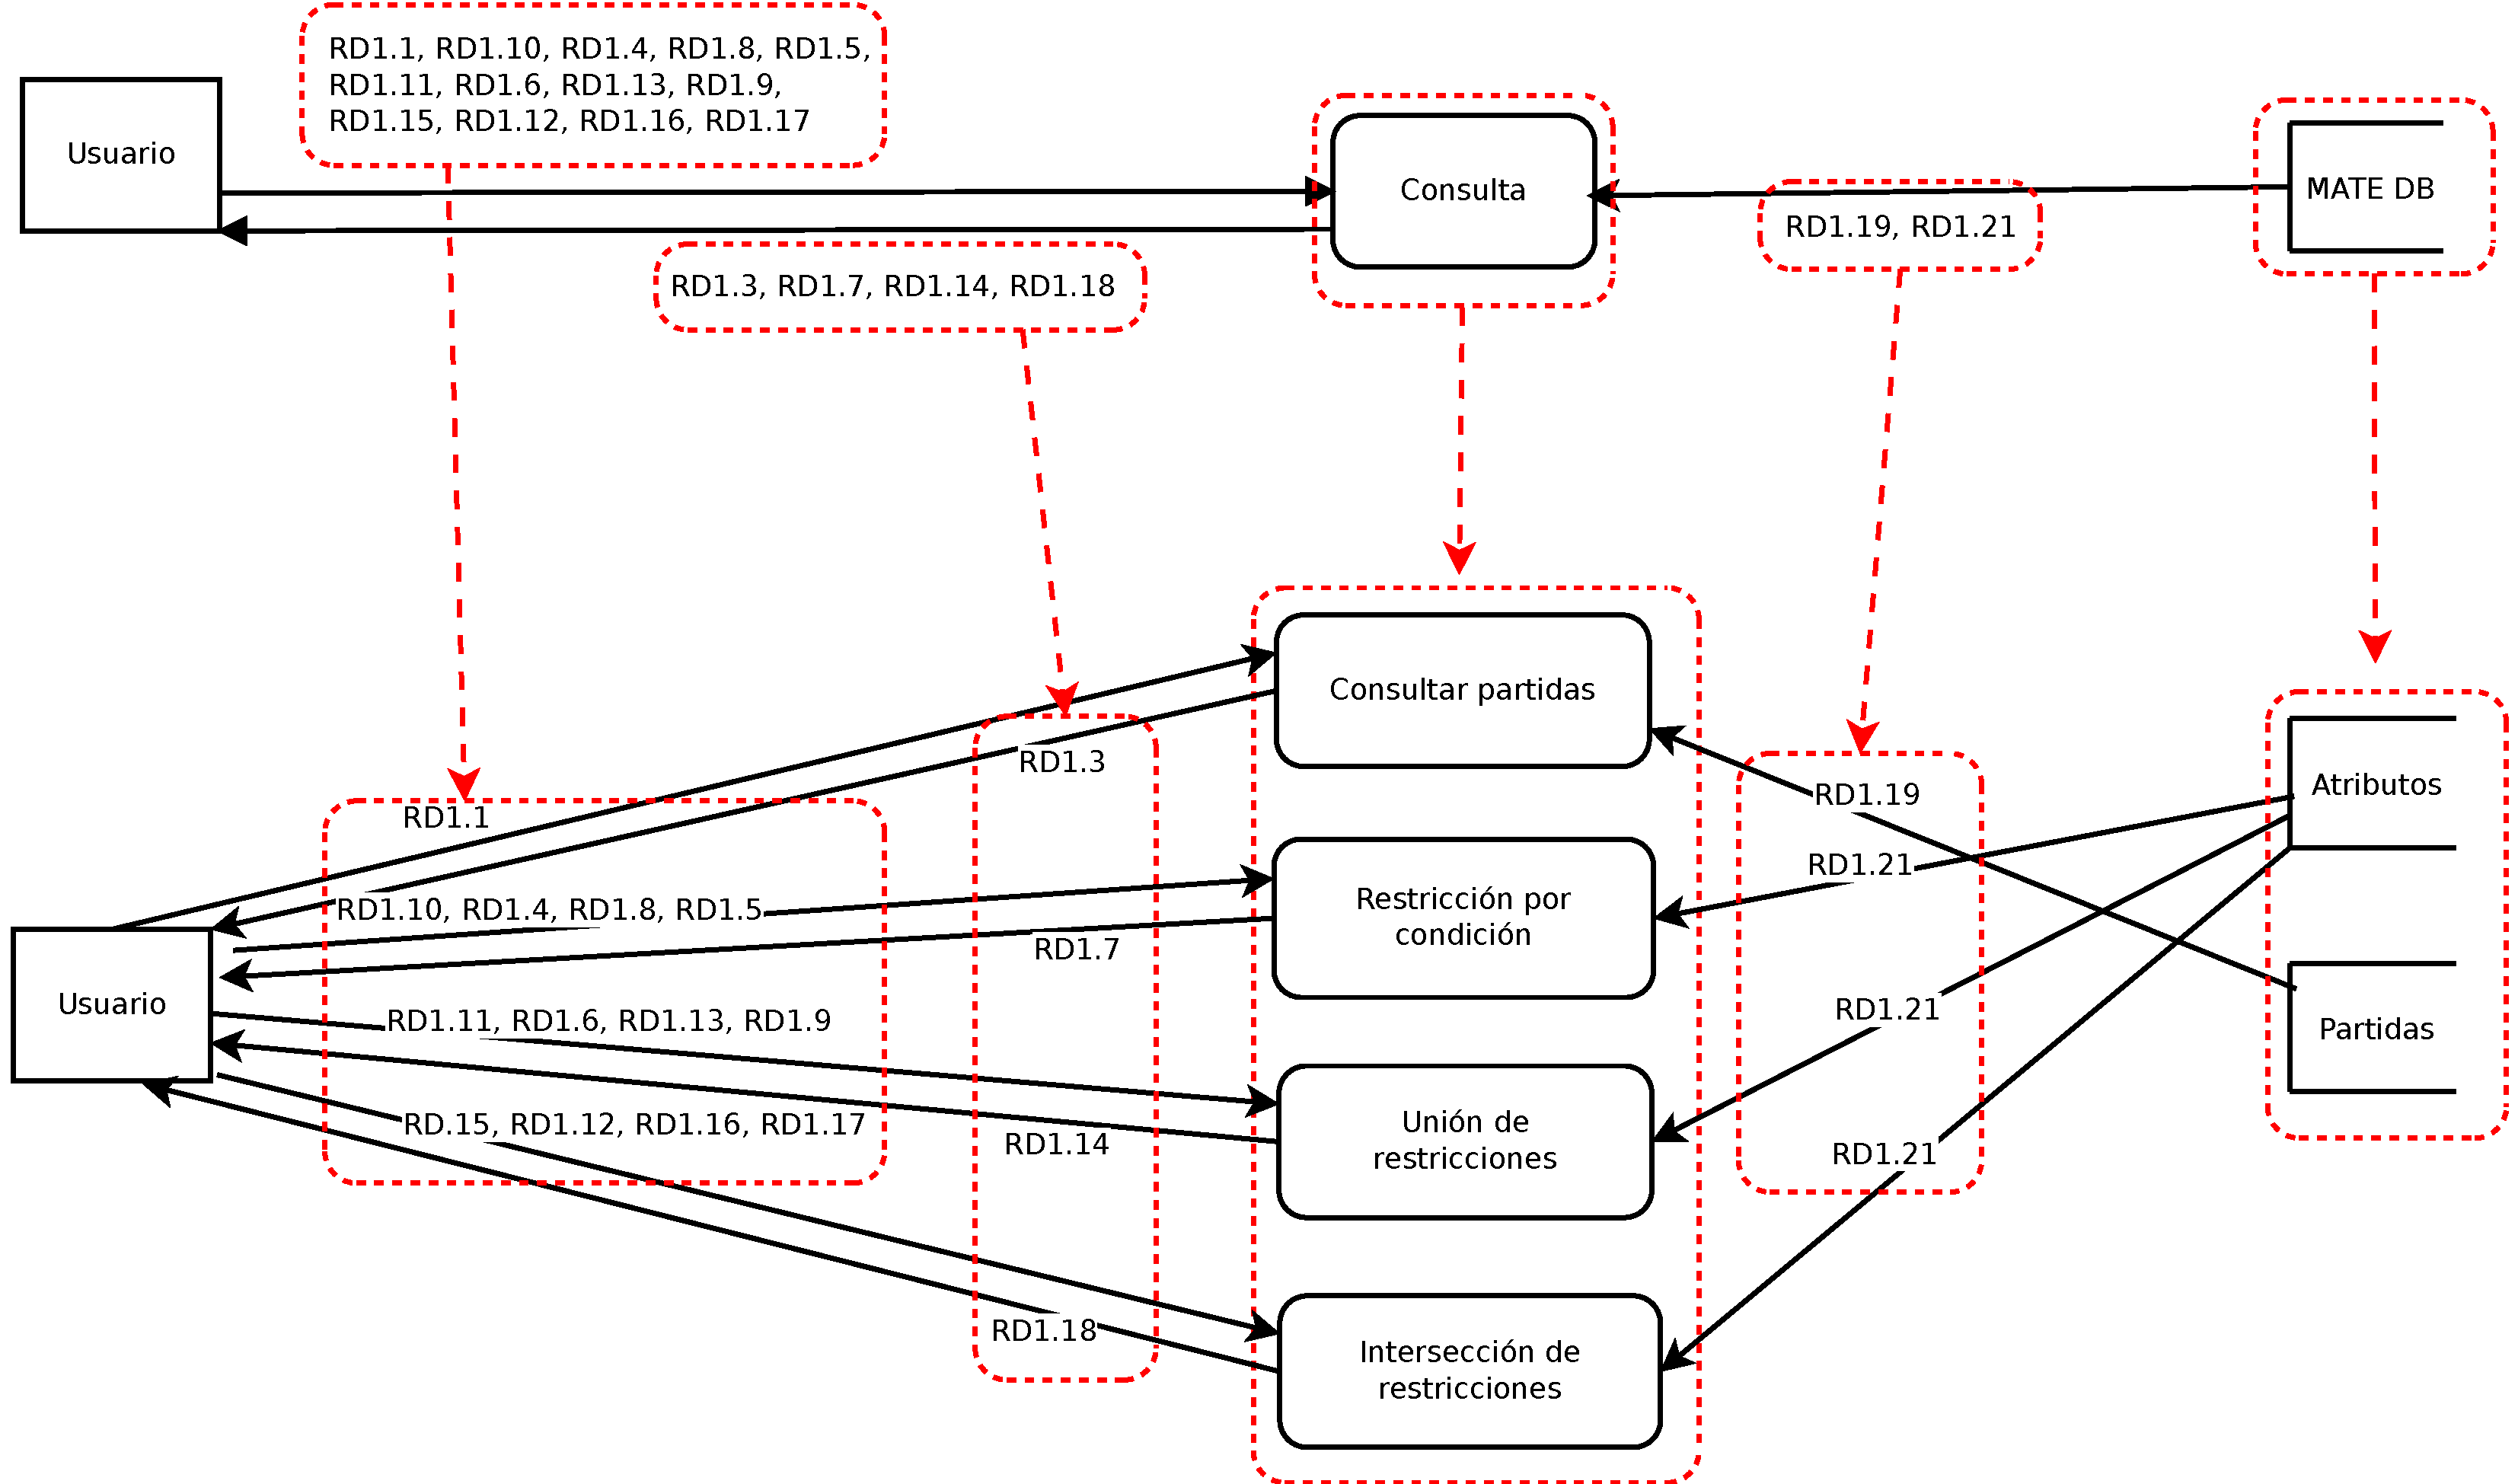
\includegraphics[width=0.7\linewidth]{../Diagramas/pdf/RefinamientoConsulta.pdf}
\caption{Flujo de datos del subsistema Consulta.}

\label{fig:RefinamientoConsulta}
\end{figure}

\subsubsection{Esquema Externo:}

\begin{figure}[h!]
	\centering
	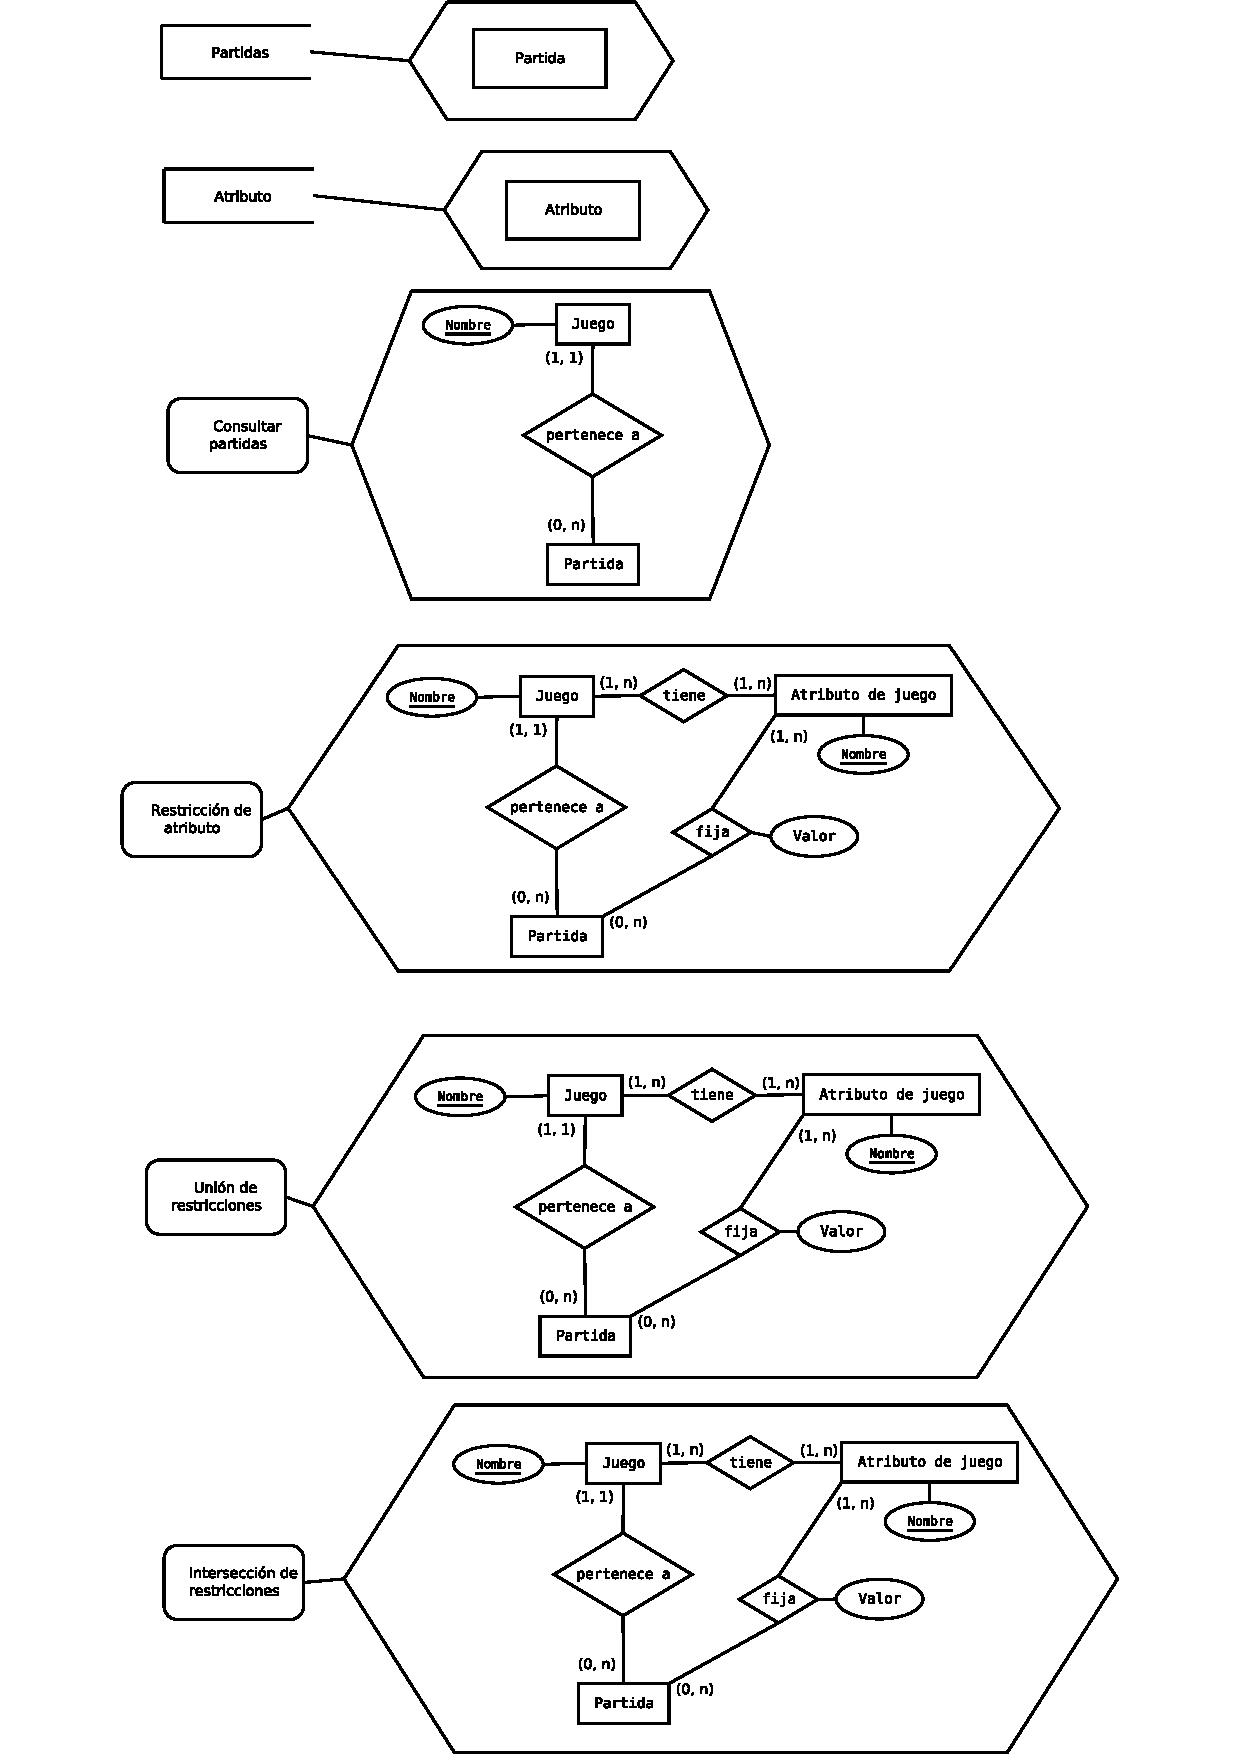
\includegraphics[width=0.7\linewidth]{../Diagramas/pdf/EsquemaExternoConsulta.pdf}
	\caption{Esquema externo de Consulta.}
	
	\label{fig:EsquemaExtConsulta}
\end{figure}
